%!TEX program = xelatex
\documentclass[12pt,titlepage,openright]{report}
\usepackage{geometry}
\geometry{a4paper}
\usepackage{graphicx}
\usepackage{amsmath}
\usepackage{amssymb}
\usepackage{url}
\usepackage{wrapfig}
\usepackage{ccaption}
\usepackage{picinpar}
\usepackage{listings}
\usepackage{multirow}
\usepackage[caption=false]{subfig}
\frenchspacing
\linespread{1.3}
\usepackage{ifxetex}
\ifxetex
  \usepackage{fontspec,xltxtra,xunicode,unicode-math}
  \usepackage{polyglossia}
  \setmainlanguage{spanish}
  \setmainfont[Mapping={tex-text},Numbers={Lining},Ligatures={Common}]{Minion Pro}
  \setsansfont[Mapping={tex-text},Colour={AA0000}]{Myriad Pro}
  \setmonofont[Mapping={tex-text},Scale={0.9}]{Inconsolata-g}
  \setmathfont[Mapping={tex-text},Numbers={Lining},Ligatures={Common}]{Minion Pro}
\else
	\usepackage[T1]{fontenc}
	\usepackage[utf8]{inputenc}
	\usepackage{lmodern}
	\usepackage[activeacute,spanish]{babel}
\fi

\begin{document}

\renewcommand\listtablename{Índice de tablas}
\renewcommand\tablename{Tabla}

\begin{titlepage}
\begin{center}
{\centering 
\includegraphics{portada.png}}
\vfill
{\LARGE UNIVERSIDAD DE MÁLAGA\\
ESCUELA TÉCNICA SUPERIOR DE\\[10pt]
INGENIEROS INDUSTRIALES}\\[25pt]
{\large DTO. DE EXPRESIÓN GRÁFICA, DISEÑO Y PROYECTOS\\
ÁREA DE EXPRESIÓN GRÁFICA EN LA INGENIERÍA}
\vfill
{\Large PROYECTO FINAL DE CARRERA\\[10pt]
ANÁLISIS DE CICLO DE VIDA DE UN ADOQUÍN}
\end{center}
\vfill
\begin{flushright}
Alumno: Francisco Pinto Oliver\\
Directora: María Luz García Ceballos\\
Ponente: José Ramón de Andrés Díaz\\
Titulación: Ingeniero Industrial
\end{flushright}
\end{titlepage}


\pagenumbering{roman} \tableofcontents \newpage \listoffigures
\newpage \listoftables \newpage \pagenumbering{arabic}

\chapter*{Agradecimientos}
\begin{flushright}
A la directora de este proyecto,\\por su inestimable ayuda.\\[10pt]
A mi familia y amigos,\\por esos buenos momentos.\\[10pt]
A María y Daniel,\\sin vosotros no sería lo mismo.
\end{flushright}
\vfill

\cleardoublepage

\part*{Memoria}
%!TEX root = informe.tex
\chapter{Introducción}
\section{Antecedentes}

La mayoría de las ciudades europeas utilizan materiales prefabricados basados en el cemento para urbanizar el terreno transformándolo en espacio público que utilizarán los ciudadanos. Estas instalaciones deben ser resistentes, económicas, funcionales y sobre todo sostenibles. La sostenibilidad es un requisito que ha ido ganando importancia en los últimos años debido no solo al aspecto económico — costes y mantenimiento principalmente — sino también al medioambiental.

El impacto medioambietal que producen las actividades humanas en la naturaleza ha pasado a ser un elemento más de estudio en cualquier proyecto de ingeniería actual. En el caso de este proyecto, el sector de las obras civiles y urbanismo supone un consumo muy elevado de materias primas y energía debido a que representa un porcentaje importante de la actividad económica de cualquier país occidental, lo que implica altas emisiones al medio ambiente.
De esta manera, utilizando la metodología de Análisis de Ciclo de Vida (ACV) se pretende conocer con una rigurosidad adecuada el ciclo de vida de un producto y/o servicio, evaluando el impacto potencial sobre el medio ambiente a lo largo de su vida.

\section{Objetivos y alcance}
El objetivo principal de este proyecto es el Análisis de Ciclo de Vida de un adoquín común utilizado en obras civiles y urbanismo. Se pretende analizar todas las entradas y salidas tanto de materiales como de energía desde la extracción de la materia prima hasta el final de vida del producto, además de identificar y clasificar los principales aspectos medioambientales y sus correspondientes impactos en los diferentes procesos que intervienen en su fabricación. De esta forma, se pueden establecer los siguientes objetivos básicos:
\begin{itemize}
\item análisis del ciclo de vida de las materias primas hasta que llegan a la planta de fabricación.
\item análisis del ciclo de vida de los procesos productivos involucrados en el proceso de fabricación hasta su salida.
\item análisis del ciclo de vida del producto hasta su final de vida.
\end{itemize}

A su vez, la redacción del presente proyecto bajo la dirección del Departamento de Expresión Gráfica, Diseño y Proyectos de la Universidad de Málaga tiene como finalidad última la obtención del título de Ingeniero Industrial.

%!TEX root = informe.tex
\chapter{Prefabricados del cemento. Adoquines}
\section{Descripción general}
A lo largo de la historia de la humanidad se han ido utilizando diferentes tipos de adoquines para pavimentar los suelos urbanos \cite{euroadoquin}. Los primeros adoquines eran de piedra, obtenidos a partir de los guijarros de río colocados sobre una capa de arena, usando una mezcla de cal y arena como sellante de juntas.

Debido al coste y el ruido del tráfico rodado, en la primera mitad del siglo XIX comenzaron a usarse los adoquines de madera, utilizando para el sellado residuos bituminosos. Debido a su reducida duración y a la posterior aparición de los neumáticos, los adoquines de madera son sustituidos por un modelo cerámico, con el que se usaba la misma arena tanto para la base como sellante.

Los adoquines de piedra seguían siendo más resistentes y además no eran tan deslizantes como los cerámicos, por lo que a finales del siglo XIX se comenzó la fabricación de los adoquines de hormigón. Estos proporcionaban una mayor uniformidad que los de piedra, eran muy resistentes y con un coste inferior. Alemania y Holanda fueron los primeros en incorporar este nuevo formato de adoquín a sus núcleos urbanos. Al principio se usaban modelos que imitaban a los de piedra tanto en forma como colocación, pero pronto se añadieron formas dentadas o curvas, permitiendo una mejor alineación con el trazado.

Finalmente, durante la década de los 70 se mejoraron sustancialmente los sistemas de fabricación, permitiendo una gran variedad de modelos de adoquines y un abaratamiento de los costes de fabricación e instalación.

\subsection{Ventajas del uso de adoquines}

En comparación con otros tipos de pavimentos tales como los asfálticos o los pavimentos contínuos hormigonados, los adoquines presentan las siguientes ventajas:

\begin{itemize}
\item Fabricación: no se utilizan derivados del petróleo, que suelen ser caros y contaminantes, además de requerir una mayor aportación de energía durante el proceso de fabricación. En contraposición, pueden utilizarse cementos y áridos locales, disminuyendo los costes de transporte.

El proceso de fabricación de los adoquines requiere una maquinaria específica debido a que son sometidos a presión y vibración para segurar una resistencia y durabilidad adecuadas. Esto implica un control sobre la fabricación, consistencia y fiabilidad del producto mayor que el resto de pavimentos.

\item Instalación: aunque los adoquines pueden colocarse de forma automatizada, están diseñados de base para ser colocados manualmente, permitiendo instalarse en zonas de difícil acceso, cargas elevadas (muelles de carga, aeropuertos, \ldots), resolver trazados complejos o pendientes pronunciadas. A diferencia de los pavimentos asfálticos, su ejecución no depende de la temperatura ambiente y pueden ser utilizados inmediatamente después de su finalización, lo que implica una reducción en los tiempos de ejecución de obra.

\item Comportamiento: los adoquines pueden ser diseñados para ser muy resistentes tanto a cargas verticales (distribuidas o puntuales) como a esfuerzos horizontales (aceleración-frenada, giros,\ldots). Además, soportan bien sin degradarse los vertidos de aceites y combustibles sobre el pavimento. Los niveles de ruido generados por el tráfico son similares o inferiores a otros pavimentos en ausencia de humedad y sensiblemente inferiores en condiciones de humedad, especialmente a bajas velocidades. La resistencia a deslizamiento es mayor al del resto de pavimentos.

\item Mantenimiento: la vida útil del adoquín viene determinada principalmente por el comportamiento de la base, subbase y explanada y no por el propio adoquín. La vida útil de cálculo suele ser a 30 años, aunque en condiciones normales puede superar los 50 años. De esta manera, al renovar el pavimento se pueden reutilizar entre un 90 y un 95\% de los adoquines originales \cite{euroadoquin}. El adoquín es la mejor opción en zonas donde aún no se han implantado todos los servicios de públicos debido a que pueden ser levantados fácilmente para llevar tareas de instalación o reparación en el subsuelo. La conservación de los adoquines se limita al relleno de juntas erosionadas con arena de sellado cada cierto tiempo y a la reposición de adoquines fracturados.

\item Costes: aunque inicialmente el precio del metro cuadrado instalado es algo superior a otros pavimentos, a largo plazo es mucho más barato debido al menor mantenimiento y la reutilización de piezas. Los pavimentos asfálticos y hormigonados requieren un mayor esfuerzo e inversión a la hora de ser reparados o retirados para acceder al subsuelo.

\item Aspecto estético: actualmente los adoquines pueden diseñarse de todas formas, texturas, colores y disposiciones según las necesidades de la obra.
\end{itemize}

\subsection{Desventajas del uso de adoquines. Otros detalles}


\section{Materias primas}
Las características de las materias primas que se pueden emplear en la fabricación de los adoquines se contemplan en la norma UNE EN 1338:2004/AC:2006. En ella se especifican detalladamente los materiaes, propiedades, requisitos y métodos de ensayo de los adoquines prefabricados de hormigón no armados y accesorios complementarios, previstos para uso peatonal, uso en áreas sometidas a tráfico de vehículos y cubiertas, como por ejemplo: aceras, límites de áreas, sendas para bicicletas, aparcamientos, carreteras, autopistas, áreas industriales, aeropuertos, estaciones de autobuses y gasolineras. Esta norma no trata la visibilidad y la tactibilidad de los adoquines ni los adoquines permeables.

\subsection{Cemento}
El cemento es un conglomerante, formado a partir de arcilla y caliza (\ce{CaCO3}), que se endure al mezclarse con agua. Para producir cemento (ver figura \ref{fig:cemento}), la arcilla y la caliza se muelen juntas. A esta mezcla se le añade yeso para conferirle la propiedad de fraguar y endurecerse. El resultado se introduce en un horno rotatorio, normalmente seco por ser más eficiente energéticamente, a una temperatura aproximada de 1450\si{\celsius}. A continuación se introduce el material en un incinerador donde el calentamiento produce la liberación del \ce{CO2} de la caliza y se produce el cemento \emph{clinker}.

\begin{center}
\ce{CaCO3 + calor -> CaO + CO2}
\end{center}

El clinker es el óxido de calcio (\ce{CaO}) obtenido de la reacción anterior, que puede encontrarse acompañado de otros minerales como hierro, aluminio o silicio. El aporte de calor necesario para obtener el clinker representa la mayor parte del coste energético en la producción de cemento.

Por último, se produce la molienda del clinker junto yeso y otros materiales (bauxita, arena,\ldots) para mejorar sus propiedades, produciendo el cemento.

\begin{figure}[!htb]
\centering
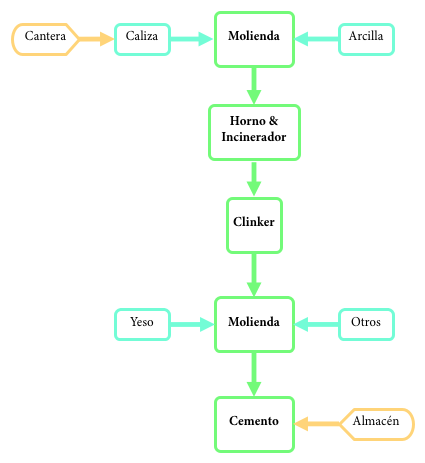
\includegraphics[width=15cm]{cemento.png}
\caption{Diagrama de flujo de la fabricación del cemento.}
\label{fig:cemento}
\end{figure}

Cuando se utiliza la palabra \emph{cemento} se refiere normalmente a un cemento tipo Portland (supone un 95\% de la producción de cementos \cite{jsjunnesson}), nombre no comercial que implica un proceso de producción y una composición característicos. De acuerdo a la norma UNE-EN 197-1:2011 \cite{une1971}, el cemento se divide en tres grupos en función de la cantidad de cemento Portland incluido: CEM I, CEM II y CEM III. El CEM I (95\% a 100\% de contenido de cemento Portland) es el más usado en la fabricación de adoquines.

Con respecto a la normativa específica de adoquines, la norma UNE 80301:1996 \cite{une80301} en el ámbito de España establece los requisitos que debe tener el cemento común. Si se utilizan cementos especiales se recurrirá a la norma UNE 80303:2013, y si son blancos a la norma UNE 80305:2012.

\subsection{Áridos}
Los áridos (entre los que se incluye la arena) son particulas de roca puede ser tanto gravas (piedras de forma natural) como macadán (piedras trituradas), teniendo cada tipo una textura diferente. Se pueden añadir diferentes tamaños de áridos para ejercer una función diferente según el mismo. Fracciones menores rellenarán las cavidades que haya entre partículas mayores, aportando adherencia a costa de un mayor peso.

El material de machaqueo para la producción de macadán se criba para eliminar las partículas menores. Debido a que las partículas que forman el macadán son más irregulares, es más fiable como material de relleno por su capacidad de incrustamiento (la grava tiene una forma más redondeada). El macadán se puede ser utilizado de forma más generalizada en función de la localización ya que la grava natural es un recurso más limitado.

La fuente de recursos de áridos son principalmente de río, mina o cantera o piedras trituradas (macadán). La granulometría de los áridos que se utilicen deberá cumplir las características indicada en la norma UNE EN 1338:2004/AC:2006.

\subsection{Agua}
El agua es muy importante en la constitución del hormigón. Reacciona químicamente con el cemento —hidratación— para proporcionar las propiedades deseadas del hormigón \cite{nrmca}. El agua de amasado es la cantidad de agua que toma contacto con el cemento y se usa para determinar las proporciones del resto de elementos para formar la mezcla. La fuerza y la durabilidad del cemento viene dado en gran parte por la cantidad de agua.

Además de su cantidad, la calidad del agua utilizada tiene efectos importantes en las propiedades del hormigón fresco, tales como el tiempo de fraguado y la facilidad de trabajo. También tiene importantes en la fuerza y durabilidad del hormigón endurecido.

\subsubsection{Fuentes posibles de agua}

Por norma general el agua adecuada para el consumo humano —agua potable— es válida. No obstante, el agua no potable puede ser utilizada siempre que no tenga un impacto negativo en las propiedades del hormigón. La mayoría de las plantas tienen una fuente de agua municipal que proporciona potable sin pruebas de calidad. En zonas rurales o en plantas portátiles in situ —instaladas y desinstaladas en el propio lugar del proyecto—, habrá que utilizar fuentes de agua no potable como ríos o masas de agua.

Otra fuente de agua es la reciclada de la limpieza —agua de lavado— de la mezcladora y otros elementos de la planta. También se podrá aprovechar el agua de precipitaciones atmosféricas que pueda recolectarse en las instalaciones de la planta.

El agua de procesado no sólo se genera de la fabricación del hormigón, sino también del lavado del hormigón reciclado. Los sistemas de recolección procesan el agua con el cemento y los áridos en forma de lechada que puede ser también utilizada como agua para la mezcla de hormigón.

Las normativas medioambientales suelen requerir que las plantas de fabricación traten y procesen tanto el agua de lluvia como el de procesado —agua de operaciones— para que adquiera ciertos niveles de pH y contenidos sólidos antes de que abandonen las instalaciones \cite{ermco}.

\subsubsection{Cualificación del agua no potable}
El agua es el recurso más importante para el ser humano. En algunas zonas el suministro de agua potable es muy escaso. El uso de fuentes de agua no potables para la producción de hormigón mantiene una producción sostenible de hormigón conservando los recursos de agua potable. La gestión del agua procedente de la producción de hormigón conforme con las normativas medioambientales representa un coste adicional para el fabricante, por lo que el uso de agua no potable representa un ahorro considerable en la producción de hormigón. Cuando se utilizan fuentes de agua no potable es importante verificar y documentar que las impurezas que contiene no merman las características del hormigón, ya que las fuentes pueden contener aceites, grasas, sales disueltas y otros elementos no controlados. Por esta razón, el fabricante debería tener en cuenta que su uso implica un coste adicional que evaluar y controlar.

\subsection{Aditivos}
Se podrán utilizar adiciones o aditivos siempre que produzcan el efecto deseado (acelerante, retardante,\ldots) y no afecte a las características esperadas del hormigón.

\section{Reciclado}
Cuando las construcciones de cemento se demuelen, el cemento es normalmente reutilizables \cite{jsjunnesson}. El cemento se transporta a una estación de reciclaje donde es triturado hasta un tamaño adecuado con la nueva utilización que se le va a dar. Puede ser empleado como material de relleno para el pavimento de nuevas carreteras o como árido en la producción de más cemento. La reutilización del cemento conlleva una disminución del uso de recursos naturales tales como la piedra o la grava.

HABLAR DEL CASO CONCRETO DE ADOQUINES Y SU RECICLADO (95\% se vuelven a usar para pavimentar. 30 años.)

%!TEX root = informe.tex
\chapter{Análisis de Ciclo de Vida: instalación, uso y mantenimiento}
%(Fuente: Manual Técnico para la correcta colocación de los Euroadoquines (MTCE 04))
\section{Introducción}
La correcta colocación y mantenimiento del pavimento con adoquines es igual de importante que la calidad en los materiales y los procesos de fabricación \cite{euroadoquinc} para que el funcionamiento del pavimento sea el adecuado.

Hay múltiples manuales y guías técnicas que explican los criterios prácticos y recomendaciones para una correcta colocación de los adoquines.

La planificación del trabajo empieza estudiando el tipo de vía y uso principal al que estará destinado el pavimento. Una vez decidido es necesario preparar la explanada y las diferentes capas componentes en función de ese uso. A continuación se coloca la capa de adoquines, se sella con arena y se realiza un vibrado del pavimento. Por último se realiza una limpieza final.

\section{Capas componentes}

\begin{itemize}
\item Explanada: Terreno natural adecuadamente compactado hasta alcanzar una capacidad portante mínima.
\item Subbase: Conjunto de capas naturales, de material granular seleccionado, estabilizado y compactado, situadas directamente sobre la explanada.
\item Base: Principal elemento portante de la estructura, situada sobre la subbase. Puede ser realizada con material granular, zahorra artificial, con un mayor grado de compactación que el alcanzado en la subbase (Base Flexible), o estar realizada con hormigón magro (Base Rígida).
\item Lecho de árido: Base de apoyo de los adoquines, destinada a absorber sus diferencias de espesor debidas a la tolerancia de fabricación, de manera que estos una vez compactados formen una superficie homogénea.
\item Adoquines: Elementos prefabricados de hormigón, cuya cara exterior, una vez colocados, forman la capa de rodadura de la superficie a pavimentar.
\item Relleno final: Una vez encastrados en el lecho de árido, sus juntas precisan un relleno final para transferir a los elementos contiguos las cargas a las que sean sometidos por acción del tráfico.
\end{itemize}

\section{Determinación de la sección tipo}\label{sec:secciontipo}

Se consideran los siguientes casos:

\begin{enumerate}
\item Viales y zonas de aparcamiento\footnote{No suelen existir zonas peatonales puras (paso eventual de vehículos de mantenimiento, limpieza y servicios).}.
\item Zonas industriales.
\end{enumerate}


Para cada caso, viales o zonas industriales, la sección puede obtenerse de forma abreviada en función de dos variables:
\begin{itemize}
\item Tipo de explanadas.
\item Categoría de tráfico.
\end{itemize}

\subsection{Tipo de explanada}

Se utiliza un sistema de clasificación de su capacidad portante mediante el índice CBR (California Bearing Ratio), indicando el tanto por ciento de la presión ejercida por un pistón sobre el suelo para alcanzar una determinada penetración baremado según un juego de muestras normalizados (ver tabla \ref{indicecbr}.

\begin{table}[!htb]
\centering
\begin{tabular}{cc}
\toprule
Calidad de la explanada & Índice CBR\\
\midrule
E1 & 5 $\leq$ CBR = 10\\
E2 & 10 $\leq$ CBR = 20\\
E3 & 20 $\leq$ CBR\\
\bottomrule
\end{tabular}
\caption{Índice CBR.}
\label{indicecbr}
\end{table}


\subsection{Categoría de tráfico}

\begin{table}[!htb]
\centering
\begin{tabular}{cc}
\toprule
Tipo & Categoría de tráfico\\
\midrule
Viales y zonas de aparcamiento & C0 \ldots C4\\
Zonas industriales & A \ldots D\\
\bottomrule
\end{tabular}
\caption{Categoría de tráfico.}
\label{categoriadetrafico}
\end{table}

\subsubsection{Categorías de tráfico en viales y zonas de aparcamiento}

Si en un área limitada existen diversos usos, a efectos de unificación se debería emplear para toda la zona la carga de cálculo más exigente.

\begin{table}[!htb]
\centering
\begin{tabular}{p{7cm}c}
\toprule
Uso previsto & Categoría de tráfico\\
\midrule
Arterias principales con gran afluencia de tráfico, paradas de bus, estaciones de servicio, etc. (50 a 149 v.p.d.) & C0\\
Arterias principales (25 a 49 v.p.d.) & C1\\
Calles comerciales con gran actividad (16 a 24 v.p.d.) & C2\\
Calles comerciales cone escasa actividad (15 v.p.d.) & C3\\
Áreas peatonales, calles residenciales & C4\\
\bottomrule
\end{tabular}
\caption{Categoría de tráfico en viales y zonas de aparcamiento.}
\label{categoriadetraficoenviales}
\end{table}


\subsubsection{Categorías de tráfico en zonas industriales}

\begin{table}[!htb]
\centering
\begin{tabular}{cccc}
\toprule
\multicolumn{2}{c}{Área} & Uso & Intensidad de uso\\
\midrule
\multirow{7}{*}{Comercial} & De operación & — & Alta\\
& \multirow{2}{*}{Almacenamiento} & Mercancia convencional & Media\\
& & Mercancía pesada & Alta\\
& Manipulación & — & Alta\\
& \multirow{3}{*}{Estacionamiento} & Vehículos pesados y ligeros & Media\\
& & Vehículos pesados exclusivamente & Alta\\
& & Semirremolques & Alta\\
\midrule
\multirow{3}{*}{Militar} & De operación & — & Alta\\
& \multirow{2}{*}{Almacenamiento} & Mercancia convencional & Media\\
& & Mercancía pesada y semirremolques & Alta\\
\midrule
\multirow{3}{*}{Pesquera} & Almacenamiento & — & Media\\
& Manipulación & — & Alta\\
& Clasificación y venta & — & Media\\
\midrule
\multirow{3}{*}{Industrial} & De operación & — & Alta\\
& \multirow{2}{*}{Almacenamiento} & Mercancia convencional & Media\\
& & Mercancía pesada & Alta\\
\bottomrule
\end{tabular}
\caption{Intensidades de uso en zonas industriales.}
\label{categoriadetraficoenzonasindustrialesintensidades}
\end{table}


\begin{table}[!htb]
\centering
\begin{tabular}{cccc}
\toprule
Intensidad de uso & \multicolumn{3}{c}{Carga de cálculo}\\
\cmidrule{2-4}
& Alta & Media & Baja\\
\midrule
Elevada & A & B & C\\
Media & A & B & D\\
Reducida & B & C & D\\
\bottomrule
\end{tabular}
\caption{Categoría de tráfico en zonas industriales.}
\label{categoriadetraficoenzonasindustriales}
\end{table}

\section{Secciones tipo}

Las secciones tipo según la base y el uso previsto del área vistas en la sección \ref{sec:secciontipo} pueden resumirse en cinco tipos para cada tipo de base, granular (figura \ref{fig:seccionestipogranular}) u hormigón magro (figura \ref{fig:seccionestipohormigon}).

\begin{figure}[!htb]
\centering
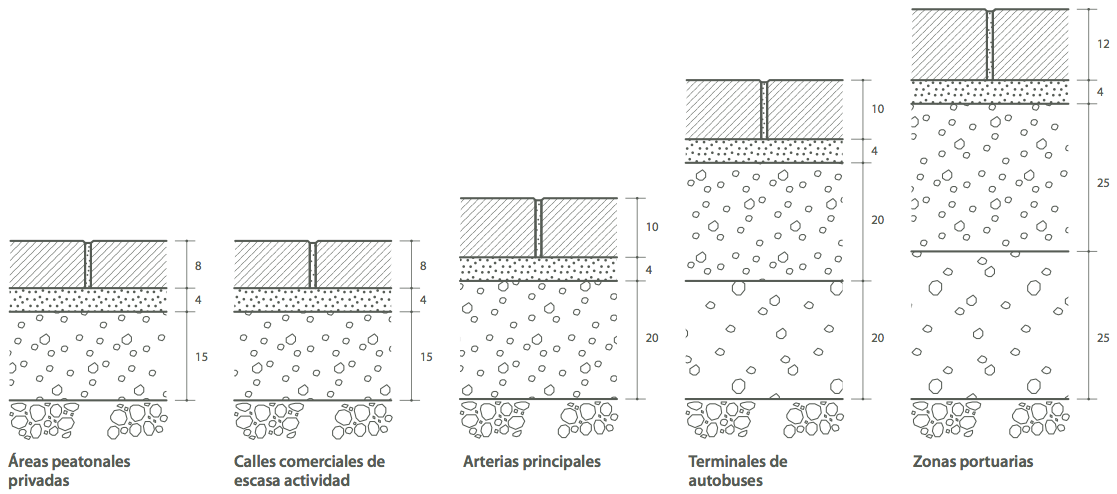
\includegraphics[width=15cm]{seccionestipo_1.png}
\caption[Secciones tipo para base granular.]{Secciones tipo para base granular. Unidades en cm. Fuente: \cite{fenollar}.}
\label{fig:seccionestipogranular}
\end{figure}

\begin{figure}[!htb]
\centering
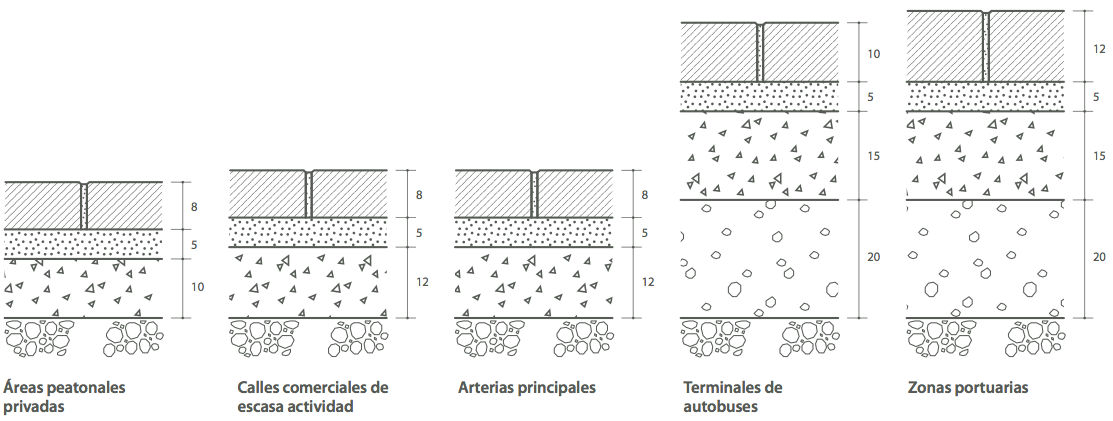
\includegraphics[width=15cm]{seccionestipo_2.png}
\caption[Secciones tipo para base de hormigón.]{Secciones tipo para base de hormigón. Unidades en cm. Fuente: \cite{fenollar}.}
\label{fig:seccionestipohormigon}
\end{figure}

\section{Modelado de los procesos}\label{sec:modeladoprocesosinstalacion}

Debido a que hay múltiples tipos de vía y uso destinado, se ha optado para el presente proyecto modelar la instalación más común, \textit{arterias principales}, que pertenece a la \textit{categoría de tráfico C1} y una \textit{calidad de explanada E2} con una base granular. Con esta clasificación, siguiendo las recomendaciones de \cite{euroadoquinc} el corte del terreno 1 \si{m^2} de superficie de terreno, que es la Unidad Funcional, será el reflejado en la tabla \ref{cortedelterreno}.

\begin{table}[!htb]
\centering
\begin{tabular}{lrrr}
\toprule
\multicolumn{4}{c}{Capas componentes para arterías principales C1-E2 con base granular}\\
\midrule
Capa componente & Grosor (\si{cm}) & Densidad (\si{kg/m^3}) & Volumen (\si{m^3})\\
\midrule
Adoquín \& Sellado & 10 & 2650 & 0.1\\
Lecho de árido & 4 & 1650 & 0.04\\
Base granular & 20 & 2560 & 0.2\\
Subbase & — & — & —\\
Explanada & \multicolumn{3}{c}{Aplanar y compactar}\\
\midrule
Total & 34 & — & 0.34\\
\bottomrule
\end{tabular}
\caption{Capas componentes para arterías principales C1-E2 con base granular.}
\label{cortedelterreno}
\end{table}

\subsection{Árido grueso para base granular (zahorra)}

Para la base granular es recomendable utilizar áridos calizos, y evitar en cualquier caso el uso de áridos con contenido en arcilla —arena de miga, arcillas refractarias—.

El acabado de la base debe ser similar al exigido para una superficie destinada a carreteras, usando una imprimación bituminosa. Tras compactar la base es recomendable hacer un sellado por medio de betún de curado rápido o emulsiones bituminosas para poder evitar filtraciones de agua a través de las juntas y que éstas dañen la base durante los primeros meses de la instalación.

La arena caliza —\textit{Limestone}, en inglés— aparece en la base de datos de SimaPro. Se pide como parámetro la masa de arena que se empleará para el rellenado. Si se tiene en cuenta que la base tiene una profundidad de 20 \si{cm} y un área de 1 \si{m^2}:

\begin{gather}
\text{Volumen de arena} = 0.2 \times 1 = 0.2 m^3\\
\rho_{arena}=2560 kg/m^3\\
\text{Masa de arena} = 0.2 \times 2560 = 512 kg
\end{gather}

Por otro lado, si se supone una distancia de entrega de 50 km hasta el destino de la instalación en un camión de transporte, se tiene:

\begin{equation}
512 kg \times 50 km = 25600 kg \times km
\end{equation}

\begin{table}[!htb]
\centering
\begin{tabular}{p{8cm}rc}
\toprule
\multicolumn{3}{c}{Arena para base granular}\\
\midrule
Materiales/ensamblajes & Cantidad & Unidad\\
\midrule
Limestone, milled, packed, at plant/CH U & 512 & \si{kg}\\
\midrule
Procesos & Cantidad & Unidad\\
\midrule
Transport, lorry 16-32t, EURO4/RER U & 25600 & \si{kg\times km}\\
\bottomrule
\end{tabular}
\caption{Modelado de la arena para base granular.}
\label{modeladoarenabase}
\end{table}

Igualmente, para la capa bituminosa de 5 cm que se aplica:

\begin{gather}
\text{Volumen de betún} = 0.05 \times 1 = 0.05 m^3\\
\rho_{betún}=1100 kg/m^3\\
\text{Masa de betún} = 0.05 \times 1100 = 55 kg
\end{gather}

Si se supone que el material proviene de una distancia de entrega de 50 km hasta el destino de la instalación en un camión de transporte, se tiene:

\begin{equation}
55 kg \times 50 km = 2750 kg \times km
\end{equation}

\begin{table}[!htb]
\centering
\begin{tabular}{p{8cm}rc}
\toprule
\multicolumn{3}{c}{Capa bituminosa para base granular}\\
\midrule
Materiales/ensamblajes & Cantidad & Unidad\\
\midrule
Bitumen sealing, at plant/RER U & 55 & \si{kg}\\
\midrule
Procesos & Cantidad & Unidad\\
\midrule
Transport, lorry 16-32t, EURO4/RER U & 2750 & \si{kg\times km}\\
\bottomrule
\end{tabular}
\caption{Modelado de la capa bituminosa para base granular.}
\label{modeladocapabituminosa}
\end{table}

\subsection{Árido semi-fino para lecho de arena}

La capa para el lecho de arena debe estar formada por áridos de resistencia geomecánica elevada, preferentemente de machaqueo ya que presentan mayores ángulos que mejoran la cohesión de la capa.

En general, los áridos deben ser poco finos, limpios y libres de elementos contaminantes.

La arena caliza —\textit{Limestone}, en inglés— aparece en la base de datos de SimaPro. Se pide como parámetro la masa de arena que se empleará para el rellenado. Si se tiene en cuenta que la base tiene una profundidad de 20 \si{cm} y un área de 1 \si{m^2}:

Sand, at mine/CH U 66
1650 kgm3
Transport 66*50

\begin{gather}
\text{Volumen de árido} = 0.04 \times 1 = 0.04 m^3\\
\rho_{arena}=1650 kg/m^3\\
\text{Masa de árido} = 0.04 \times 1650 = 66 kg
\end{gather}

Por otro lado, si se supone una distancia de entrega de 50 km hasta el destino de la instalación en un camión de transporte, se tiene:

\begin{equation}
66 kg \times 50 km = 3300 kg \times km
\end{equation}

\begin{table}[!htb]
\centering
\begin{tabular}{p{8cm}rc}
\toprule
\multicolumn{3}{c}{Árido semi-fino para lecho de arena}\\
\midrule
Materiales/ensamblajes & Cantidad & Unidad\\
\midrule
Gravel, crushed, at mine/CH U & 66 & \si{kg}\\
\midrule
Procesos & Cantidad & Unidad\\
\midrule
Transport, lorry 16-32t, EURO4/RER U & 3300 & \si{kg\times km}\\
\bottomrule
\end{tabular}
\caption{Modelado del árido semi-fino para lecho de arena.}
\label{modeladoaridosemifino}
\end{table}

\subsection{Arena para sellado}

La arena para sellado debe ser una arena sin exceso de finos, ya que si existen demasiados finos, se producirá un vaciado de las juntas con el uso y limpieza del pavimento o bien se filtrarás hacia el lecho.

Además debe ser libre de sales solubles y otros contaminantes, ya que pueden provocar la aparición de eflorescencias —igual que en el caso del lecho de árido—.

No se debe usar mortero para el sellado de las juntas, ya que no se podrán retirar para hacer tareas de mantenimiento —principal ventaja de los adoquines de hormigón—, además de perder flexibilidad del conjunto.

La arena de sílice —\textit{Silica sand}, en inglés— es un material adecuado para esta tarea \cite{website:cement}. SimaPro pide como parámetro la masa de arena que se empleará para el rellenado. Si se tiene en cuenta que el adoquín mide 10 \si{cm} de altura, 1 \si{cm} quedará enterrado en el lecho, y se añadirá 1 \si{cm} por encima para el vibrado; por otro lado, la junta medirá 5 \si{mm}, se puede obtener el volumen y a partir de él la masa:

\begin{gather}
1 m^2 = 50 \text{ adoquines} = 10 \times 5\\
Adoquin = 20 \times 10 \times 6 cm\\
\delta_{junta} = 0.5cm\\
Largo = 10 \times 10 + 9 \times 0.5 = 104.5 cm\\
Ancho = 5 \times 20 + 4 \times 0.5 = 102 cm\\
\text{Superficie de arena} = 104.5 \times 0.5 + 102 \times 0.5 = 103.25 cm^2\\
\text{Volumen de arena} = 103.25 \times 10 = 1032.5 cm^3\\
\rho_{arena}=2.6 g/cm^3\\
\text{Masa de arena} = 1032.5 \times 2.65 = 2.74 kg
\end{gather}

Por otro lado, si se supone una distancia de entrega de 50 km hasta el destino de la instalación en un camión de transporte, se tiene:

\begin{equation}
2.74 kg \times 50 km = 137 kg \times km
\end{equation}

\begin{table}[!htb]
\centering
\begin{tabular}{p{8cm}rc}
\toprule
\multicolumn{3}{c}{Arena para sellado}\\
\midrule
Materiales/ensamblajes & Cantidad & Unidad\\
\midrule
Silica sand, at plant/DE U & 2.74 & \si{kg}\\
\midrule
Procesos & Cantidad & Unidad\\
\midrule
Transport, lorry 16-32t, EURO4/RER U & 137 & \si{kg\times km}\\
\bottomrule
\end{tabular}
\caption{Modelado de la arena para sellado.}
\label{modeladoarenasellado}
\end{table}

\subsection{Excavación del terreno}

A la hora de realizar un pavimento de adoquines, se debe realizar en primer lugar la excavación del terreno. Dado que el grosor total de las capas componentes es de 34 \si{cm} y se dispone de un área de 1 \si{m^2}, el volumen a introducir para el modelo será 0.34 \si{m^3}, utilizando como entrada de SimaPro de excavación con herramienta hidráulica, \textit{Excavation, hydraulic digger}.

\begin{table}[!htb]
\centering
\begin{tabular}{p{8cm}rc}
\toprule
\multicolumn{3}{c}{Excavación del terreno}\\
\midrule
Materiales/combustibles & Cantidad & Unidad\\
\midrule
Excavation, hydraulic digger/RER U & 0.34 & \si{m^3}\\
\bottomrule
\end{tabular}
\caption{Modelado de la excavación del terreno.}
\label{modeladoexcavacion}
\end{table}

\subsection{Compactación de la explanada}

Una vez excavado el terreno es necesario compactar lo que será la explanada. La bibliografía consultada no ha ofrecido ninguna solución óptima a este tipo de proceso, por lo que se ha optado por asemejar el tipo de trabajo de un tractor usando un rodillo para cultivar la tierra —\textit{Tillage, rolling}, en inglés— con el rodillo utilizado por una apisonadora o compactadora —\textit{road roller}, en inglés—. En este caso, la compactación se realiza en unidades de área, por lo que se ha introducido 1 \si{m^2} de superficie.

\begin{table}[!htb]
\centering
\begin{tabular}{p{8cm}rc}
\toprule
\multicolumn{3}{c}{Compactación de la explanada}\\
\midrule
Materiales/combustibles & Cantidad & Unidad\\
\midrule
Tillage, rolling/CH U & 1 & \si{m^2}\\
\bottomrule
\end{tabular}
\caption{Modelado de la compactación de la explanada.}
\label{modeladoexplanada}
\end{table}

\subsection{Compactación de la capa base}

En el caso de arterias principales no existe una capa subbase, por lo que se procederá a la extensión y compactación de la capa base. Una correcta ejecución es fundamental ya que esta capa es el principal elemento portante de la estructura y se encarga de transmitir hacia la explanada las cargas verticales. El espesor de esta base debe ser uniforme.

Es muy importante que el plano de la capa base respete una pendiente mínima del 1\% para permitir un drenaje adecuado de las aguas superficiales sin que provoquen daños a las capas portantes, y así evitar daños en la superficie.

La bibliografía consultada no ha ofrecido ninguna solución óptima a este tipo de proceso, por lo que se ha optado por asemejar el tipo de trabajo de un tractor usando un rodillo para cultivar la tierra —\textit{Tillage, rolling}, en inglés— con el rodillo utilizado por una apisonadora o compactadora —\textit{road roller}, en inglés—. En este caso, la compactación se realiza en unidades de área, por lo que se ha introducido 1 \si{m^2} de superficie.

\begin{table}[!htb]
\centering
\begin{tabular}{p{8cm}rc}
\toprule
\multicolumn{3}{c}{Compactación de la capa base}\\
\midrule
Materiales/combustibles & Cantidad & Unidad\\
\midrule
Tillage, rolling/CH U & 1 & \si{m^2}\\
\bottomrule
\end{tabular}
\caption{Modelado de la compactación de la capa base.}
\label{modeladocapabase}
\end{table}

\subsection{Compactación del lecho de árido}

El lecho de árido es, junto con la calidad del adoquín, el elemento fundamental que determina el comportamiento y durabilidad del pavimento. El lecho se extiende directamente sobre la capa base.

Una de las funciones principales es la de absorber las pequeñas diferencias de espesor de los adoquines siguiendo las tolerancias de la normativa \cite{une1338}, de forma que, una vez se hace la compactación de los adoquines, formen un plano de rodadura uniforme que transmita las cargas del tráfico sin deteriorar las piezas.

Otra de las funciones del lecho de árido es la de actuar como elemento de relleno inferior de las juntas de los adoquines. Al ser compactados los adoquines, quedan incrustados en el lecho, y así se evita el contacto directo entre las caras laterales de las piezas.


Al igual que en las compactaciones anteriores, la bibliografía consultada no ha ofrecido ninguna solución óptima a este tipo de proceso, por lo que se ha optado por asemejar el tipo de trabajo de un tractor usando un rodillo para cultivar la tierra —\textit{Tillage, rolling}, en inglés— con el rodillo utilizado por una apisonadora o compactadora —\textit{road roller}, en inglés—. En este caso, la compactación se realiza en unidades de área, por lo que se ha introducido 1 \si{m^2} de superficie.

\begin{table}[!htb]
\centering
\begin{tabular}{p{8cm}rc}
\toprule
\multicolumn{3}{c}{Compactación del lecho de árido}\\
\midrule
Materiales/combustibles & Cantidad & Unidad\\
\midrule
Tillage, rolling/CH U & 1 & \si{m^2}\\
\bottomrule
\end{tabular}
\caption{Modelado de la compactación del lecho de árido.}
\label{modeladolecho}
\end{table}

\subsection{Sellado con arena y vibrado del pavimento}

Una vez colocados y alineados los adoquines de forma que el lecho de árido también sirva de separador entre las juntas, se extiende sobre el pavimento una capa ligera de arena para completar el espacio.

La importancia de esta etapa yace en que un relleno completo de las juntas hace que tanto esta arena como el árido del leche sean los transmisores de los esfuerzos laterales entre los adoquines. Si el pavimento soporta tráfico sin haber sido bien sellado, se pueden producr daños importantes sobre el mismo.

El sellado consiste en extender arena fina y seca sobre el pavimento e introducirla entre las juntas con un barrido manual o mecánico, intentando que quede una ligera capa de excedente sobre toda la superficie.

A continuación se realiza un proceso de compactación sobre el pavimento para garantizar un relleno adecuado de las juntas. Esta compactación se puede realizar bien con placas vibrantes —\textit{vibratory plates} o \textit{plate compactor}, en inglés— o con rodillos mecánicos con vibración. La fuerza vibratoria y el peso de las herramientas deben ser proporcionales al tipo de pavimento que se está ejecutando.

Una vez se realiza la compactación, el pavimento puede ponerse en servicio inmediatamente.

El proceso de compactación no aparece reflejado en las librerías que proporciona SimaPro. De acuerdo a \cite{rieradevall}, las placas vibrantes para compactar pueden modelarse mediante su consumo de combustible. En concreto 2.43 \si{MJ} de gasoil para 1 ft$^2$. Por lo que, extrapolando para 1 \si{m^2}, se tendría:

\begin{equation}
2.43\frac{MJ}{{ft}^2} \times \frac{10.764{ft^2}}{1m^2}=26.16MJ/m^2
\end{equation}

\begin{table}[!htb]
\centering
\begin{tabular}{p{8cm}rc}
\toprule
\multicolumn{3}{c}{Vibrado del pavimento}\\
\midrule
Materiales/combustibles & Cantidad & Unidad\\
\midrule
Diesel, burned in building machine/GLO U & 26.16 & \si{MJ}\\
\bottomrule
\end{tabular}
\caption{Modelado del vibrado del pavimento.}
\label{modeladovibrado}
\end{table}

\subsection{Limpieza final}

Cuando se ha terminado el vibrado del pavimento y se ha observado que las juntas quedan completamente rellenas, se debe iniicar el proceso de limpieza de la superficie para eliminar la arena de sellado excedente.

Esta limpieza se realiza mediante un barrido manual, dejando una pequeña capa de arena sobre el pavimento para que el tráfico termine de colocar sobre las juntas de forma natural. Una vez finalizada la limpieza se puede abrir la vía al uso destinado.

Este proceso no se ha incluido en SimaPro ya que es un trabajo manual de un operario y no se consumen directamente materiales o combustibles.

\section{Modelado completo}

Los modelos de los procesos explicados en la sección \ref{sec:modeladoprocesosinstalacion} han sido introducidos en SimaPro para crear un modelo completo que represente la instalación de un metro cuadrado de adoquín modelo Holanda 6. El listado completo de procesos se muestra en la tabla \ref{modeladocompletoinstalacion}.

\begin{table}[!htb]
\centering
\begin{tabular}{p{8cm}rc}
\toprule
\multicolumn{3}{c}{Fabricación 1 \si{m^2} adoquín Holanda 6}\\
\midrule
Materiales/ensamblajes & Cantidad & Unidad\\
\midrule
Árido grueso para base granular (zahorra) & 1 & p\\
Capa bituminosa para base granular (zahorra) & 1 & p\\
Árido semi-fino para lecho de arena & 1 & p\\
Arena para sellado de juntas & 1 & p\\
\midrule
Procesos & Cantidad & Unidad\\
\midrule
Excavación del terreno para arteria principal C1-E2 & 1 & p\\
Compactación de la explanada & 1 & p\\
Compactación de la capa base & 1 & p\\
Compactación del lecho de arena & 1 & p\\
Sellado+vibrado del pavimento & 1 & p\\
\bottomrule
\end{tabular}
\caption{Modelado completo de la instalación.}
\label{modeladocompletoinstalacion}
\end{table}

\section{Resultados}

Una vez creado el modelo completo del proceso de instalación, SimaPro genera un análisis de los datos introducidos. El método de análisis elegido es \textit{ReCiPe Endpoint (H) V1.06 / Europe ReCipe H/A}, previamente explicado en la sección \ref{sec:recipe}.

\begin{figure}[!htb]
\centering
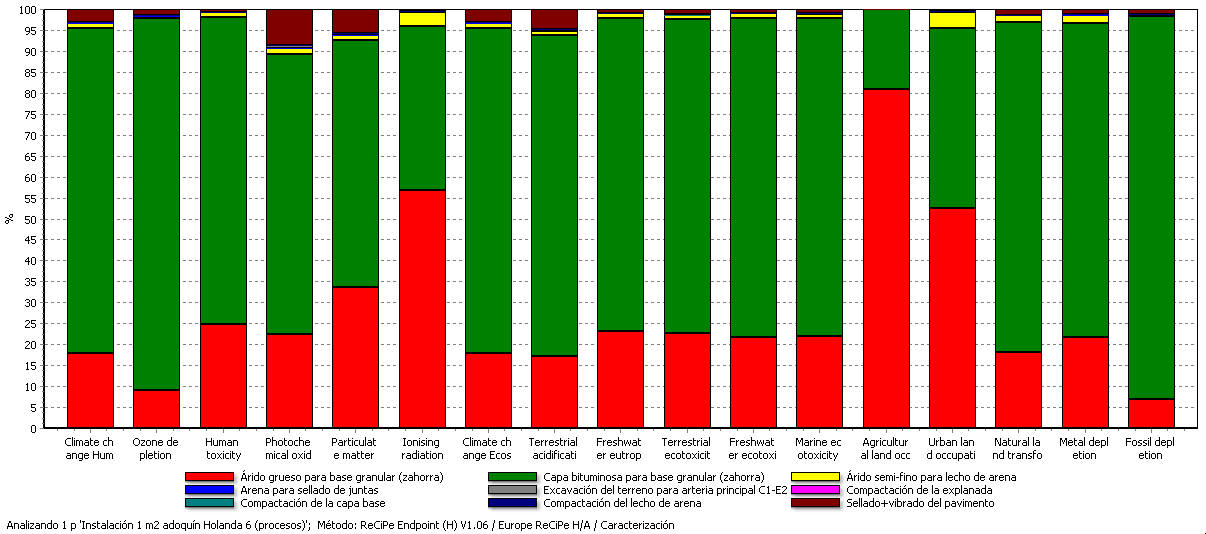
\includegraphics[angle=90,height=19cm]{instalacion_caracterizacion.png}
\caption{Caracterización del análisis de instalación de 1 \si{m^2} de adoquín.}
\label{fig:caracterizacioninstalacion}
\end{figure}

\begin{figure}[!htb]
\centering
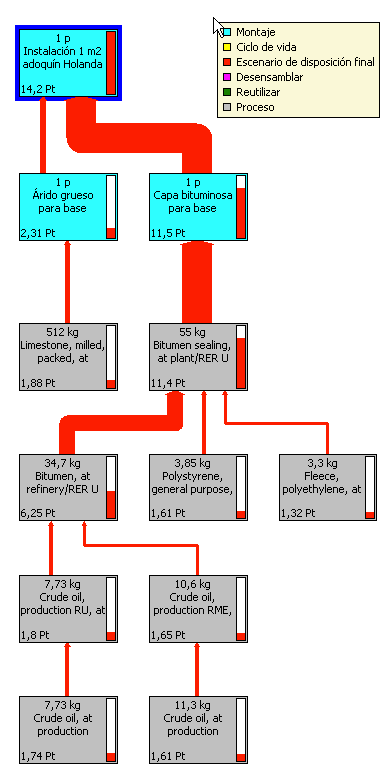
\includegraphics[height=19cm]{instalacion_red.png}
\caption{Red del análisis de instalación de 1 \si{m^2} de adoquín.}
\label{fig:redinstalacion}
\end{figure}

\cleardoublepage

\part*{Pliego de condiciones}
%!TEX root = informe.tex

\setcounter{chapter}{0}
\chapter{Condiciones técnicas}
% \addcontentsline{toc}{chapter}{Condiciones técnicas}

\section{Generalidades}

Los principios del Análisis de Ciclo de Vida son fundamentales y se deberán utilizar como orientación para tomar decisiones relacionadas tanto con la planificación como con la realización del análisis.

\section{Apreciación general del ciclo de vida}

El Análisis de Ciclo de Vida considerará el ciclo de vida completo del producto, desde la extracción y adquisición de la materia prima, pasando por la producción de energía y materia, y la fabricación, hasta el uso y el tratamiento al final de la vida útil y la disposición final. A través de esta visión general, se identificará y intentará evitar el desplazamiento de una carga ambiental potencial entre las etapas del ciclo de vida o los procesos individuales.

\section{Enfoque ambiental}
El Análisis de Ciclo de Vida tratará los aspectos e impactos ambientales del sistema del producto. Los aspectos e impactos económicos y sociales estarán fuera del alcance del Análisis de Ciclo de Vida. Se podrán combinar otras herramientas con el Análisis de Ciclo de Vida para análisis más profundos.

\section{Enfoque relativo y Unidad Funcional}
El Análisis de Ciclo de Vida será un enfoque relativo, que se estructurará alrededor de una Unidad Funcional. Esta Unidad Funcional definirá el estudio. Todos los análisis subsecuentes serán, por tanto, relativos a esa Unidad Funcional, ya que todas las entradas y salidas en el Inventario de Ciclo de Vida (ICV), y consecuentemente el perfil de la Evaluación del Impacto del Ciclo de Vida (EICV), se relacionarán con la Unidad Funcional.

\section{Enfoque iterativo}
El Análisis de Ciclo de Vida será una técnica iterativa. Las fases individuales del Análisis de Ciclo de Vida utilizarán resultados de las otras fases. El enfoque iterativo en y entre las fases contribuirá a la integridad y coherencia del estudio y de los resultados presentados.

\section{Transparencia}
Debido a la complejidad inherente al Análisis de Ciclo de Vida, la transparencia será un principio guía importante en la realización del Análisis de Ciclo de Vida, a fin de asegurar una adecuada interpretación de los resultados.

\section{Integridad}
El Análisis de Ciclo de Vida considerará todos los atributos o aspectos del entorno natural, de la salud humana y de los recursos. La consideración en un único estudio y con una perspectiva transversal de todos los atributos y aspectos, se podrán identificar y evaluar las compensaciones potenciales.

\section{Prioridad del enfoque científico}
Las decisiones en el Análisis de Ciclo de Vida se basarán preferentemente en las ciencias naturales. Si esto no es posible, se podrán utilizar otros enfoques, como las ciencias económicas y sociales, o se puede hacer referencia a convencio- nes internacionales. Si no existiera una base científica ni una justificación basada en otros enfoques o en convenciones internacionales, las decisiones se podrán basar en juicios de valor.

\section{Alcance}
Cuando se defina el alcance del Análisis de Ciclo de Vida, se considerará el contexto de la toma de decisión; es decir, los sistemas del producto estudiados deberán tratar adecuadamente los productos y procesos afectados por la aplicación prevista.

Los ejemplos de aplicación se referirán a decisiones que pretendan conseguir mejoras ambientales, lo que también constituye el enfoque global de la serie ISO 14000. Por lo tanto, los productos y procesos estudiados en un Análisis de Ciclo de Vida son aquellos afectados por la decisión que el Análisis de Ciclo de Vida pretende apoyar.

\chapter{Condiciones administrativas y legales}
% \addcontentsline{toc}{chapter}{Condiciones administrativas y legales}

\section{Autoría}
El autor de este proyecto cede al 50\% los derechos derivados de este proyecto al Departamento de Expresión Gráfica, Diseño y Proyectos de la Escuela Técnica Superior de Ingeniería Industrial de la Universidad de Málaga.

\section{Realización y supervisión}
El presente proyecto será realizado por el autor del mismo, bajo dirección y supervisión del tutor. Si esto no fuera posible, dicha realización y asesoría debería ser llevada a cabo por personal del Departamento de Expresión Gráfica, Diseño y Proyectos de la Escuela Técnica Superior de Ingeniería Industrial de la Universidad de Málaga.

\section{Cambios y desarrollos posteriores}
El autor del presente proyecto deberá ser puntualmente informado de los posibles cambios o modificaciones que pudiesen realizarse en el mismo.

En el caso de cambios o desarrollos posteriores de este proyecto se informará al autor para colaborar en el estudio o investigación que se este realizando.

\section{Consultas}
Se autoriza la consulta de este proyecto a toda persona autorizada por parte del Departamento de Expresión Gráfica, Diseño y Proyectos y a cualquier persona matriculada en la Universidad de Málaga que podrá solicitar el Proyecto en la Biblioteca de la Escuela Técnica Superior de Ingeniería Industrial de la Universidad de Málaga.

\vspace{1cm}
\today \hfill Fdo. Francisco José Pinto Oliver

\cleardoublepage

\appendix
\chapter{Planos}\label{aped.A}
En este apéndice se incluyen los planos de la planta de fabricación de materiales prefabricados y los modelos de fabricación del adoquín y su molde.
\cleardoublepage

%!TEX root = informe.tex
\addcontentsline{toc}{chapter}{Bibliografía}
% \bibliographystyle{alpha} % BibTeX
% \bibliography{informe}
\begin{thebibliography}{100}

% \bibitem[PFULL97]{pfullana}
% Fullana, P. y Puig, R., \emph{Análisis de Ciclo de Vida}, Editorial Rubens, Barcelona (España), 1997.

% \bibitem[MLGAR13]{mlgceballos}
% García Ceballos, M. L., \emph{Tésis Doctoral. Análisis de Ciclo de Vida de Puntos de Luz de Alumbrado Exterior}, Universidad de Málaga, Málaga (España), 2013, pp.56.

% \bibitem[MGOED10]{mgoedkoop}
% Goedkoop, M. et al., \emph{SimaPro 7 Tutorial}, Pré Consultants, Amersfoort (Holanda), 2010, disponible en \url{http://http://www.pre-sustainability.com/manuals}.

\bibitem[MALAK09]{malak09}
Malaka de Prefabricados, \emph{Ficha Técnica de Adoquines de Hormigón}, Málaga (España), 2009.

% \bibitem[NJUNG11]{mnjungbluth}
% Jungbluth, N. et al., \emph{Environmetal Impacts of Swiss Consumption and Production}. Federal Office for the Environment, Ginebra (Suiza), 2011.

% \bibitem[JSJUN05]{jsjunnesson}
% Sjunnesson, J., \emph{Life Cycle Assessment of Concrete Master Thesis}, Environmental and Energy Systems Studies, Lund University, Lund (Suecia), 2005.

% \bibitem[ISO14040]{iso14040}
% International Organization for Standardization, \emph{UNE-EN-ISO 14040:2006, Gestión Ambiental. Análisis de ciclo de vida. Principios y marco de referencia}, AENOR, Madrid (España), 2006.

% \bibitem[ISO14440]{iso14440}
% International Organization for Standardization, \emph{UNE-EN-ISO 14440:2006, Gestión ambiental. Análisis de ciclo de vida. Requisitos y Directrices}, AENOR, Madrid (España), 2006.

% \bibitem[ISO150041]{iso150041}
% International Organization for Standardization, \emph{UNE-EN-ISO 150041EX:1998, Análisis de ciclo de vida simplificado}, AENOR, Madrid (España), 2006.

% \bibitem[UNE127338]{une127338}
% Una Norma Española, \emph{UNE 127338:2007 Propiedades y condiciones de suministro y recepción de los adoquines de hormigón. Complemento nacional a la Norma UNE-EN 1338.}, AENOR, Madrid (España), 2007.

% \bibitem[CARVA01]{carva01}
% de Carvalho Filho, A.C., \emph{Tésis Doctoral de Análisis del ciclo de vida de productos derivados del cemento. Aportaciones al análisis de inventarios del ciclo de vida del cemento}, E.T.S. Ingenieros de Caminos, Canales y Puertos, Universidad Politécnica de Cataluña, Barcelona (España), 2001.

% \bibitem[TRINI99]{trini99}
% Trinius, W., \emph{Environmental Assessment in Building and Construction. Goal and Scope Definition as Key to Methodology choices PhD. Thesis}, Kunliga Tekniska Högskolna, Estocolmo (Suecia), 1999.

% \bibitem[UNE1338]{une1338}
% Una Norma Española, \emph{UNE-EN 1338:2004/AC:2006 Adoquines de hormigón. Especificaciones y métodos de ensayo.}, AENOR, Madrid (España), 2006.

% \bibitem[EADMT04]{eadmt04}
% Asociación Española para la Investigación y Desarrollo del Adoquín de Hormigón, \emph{Manual Técnico del Euroadoquín, MTE-04}, Madrid (España), 2004.

% \bibitem[EADMC04]{eadmc04}
% Asociación Española para la Investigación y Desarrollo del Adoquín de Hormigón, \emph{Manual Técnico para la correcta colocación de los Euroadoquines, MTCE-04}, Madrid (España), 2004.

% \bibitem[UNE1971]{une1971}
% Una Norma Española, \emph{UNE-EN 197-1:2011 La norma europea de especificaciones de cementos comunes.}, AENOR, Madrid (España), 2011.

% \bibitem[UNE80301]{une80301}
% Una Norma Española, \emph{UNE 80301:1996 Cementos. Cementos comunes. Composición, especificaciones y criterios de conformidad.}, AENOR, Madrid (España), 1996.

% \bibitem[ANDEC13]{andec13}
% Asociación Nacional de la Industria del Prefabricado de Hormigón (ANDECE), \emph{Los prefabricados de hormigón}, Madrid (España), consultado el 03-07-2013, disponible en \url{http://www.andece.org}.

\bibitem[IECA13]{ieca13}
Instituto Español del Cemento y sus Aplicaciones (IECA), \emph{Guías Técnicas}, Madrid (España), consultado el 24-07-2013, disponible en \url{http://www.ieca.es/lstFichas.asp?id_cat=113}.

\bibitem[ALBER12]{alber12}
Prefabricados Alberdi, \emph{Preguntas frecuentes}, Vizcaya (España), consultado el 28-06-2013, disponible en \url{http://www.prefabricadosalberdi.com/alberdi/dm/faq.asp?nombre=2370&hoja=0&sesion=1}
\end{thebibliography}


\end{document}
